\documentclass[12pt]{article}



%Paquetes a utilizarse
\usepackage[width=7in, height=9.5in, top=0.75in, papersize={8.5in,11in}]{geometry}
\usepackage[spanish]{babel} 
\decimalpoint
\usepackage[utf8]{inputenc}
\usepackage{bbding}
\usepackage[colorlinks = true, linkcolor = blue, urlcolor = BlueViolet, citecolor = OliveGreen]{hyperref}
\usepackage{graphicx}
\usepackage{amssymb,amsthm,amsmath}
\usepackage{enumerate}
\usepackage{array,multicol,multirow}
\usepackage{xcolor}
\usepackage{fancybox,tcolorbox}
\usepackage{caption,subcaption,float,tabularx}
\usepackage{enumitem}

\theoremstyle{definition}
\newtheorem{corolario}{Corolario}
\newtheorem{lema}[corolario]{Lema}
\newtheorem{proposicion}[corolario]{Proposición}
\newtheorem{teorema}[corolario]{Teorema}
\newtheorem{propiedad}[corolario]{Propiedad}
\newtheorem*{observacion}{Observación}
\newtheorem{definicion}{Definición}
\newtheorem*{demostracion}{Demostración}
\newtheorem{ejemplo}{Ejemplo}
\newtheorem{problema}{Problema}
\newtheorem*{solucion}{Solución}
\newtheorem{ejercicio}{\PencilRightDown \  Ejercicio}
\newtheorem{step}{Paso}
\newtheorem{credito}{Crédito}

\usepackage{tikz}
\usetikzlibrary{arrows.meta,babel,calc,positioning}

\renewcommand{\arraystretch}{1.5}
\providecommand{\abs}[1]{\lvert#1\rvert}
\providecommand{\norm}[1]{\lVert#1\rVert}

\renewcommand{\tabularxcolumn}[1]{m{#1}}
\newcommand{\Evaluacion}[4]{
\setcounter{ejercicio}{0}
\noindent\begin{tabular}{lcr}
	\includegraphics[height=3cm]{Logos/logo-UES.png}\hspace{2.5em}
	&
	\includegraphics[height=2.75cm]{Logos/logo-PJT.png}
	& 
	\hspace{2.5em}\includegraphics[height=2.75cm]{Logos/logo-MINEDUCYT.png}
\end{tabular}

\hfill

\begin{center}
    
    UNIVERSIDAD DE EL SALVADOR
    \\PROGRAMA JÓVENES TALENTO
    \\FDTC 2022
    \\#2
    \\Nivel Olímpico C de Matemáticas

\end{center}

\begin{center}
    #1
\end{center}

%\textbf{Nombre}: \enspace\hrulefill

#3

\input{#4}
\newpage
}

\newtheorem{obs}{Observación}

%\usepackage[margin=2.5cm]{geometry}
%\usepackage{wasysym}
%\usepackage{stmaryrd,textcomp}
%\usepackage{pgf,tikz}
%\usetikzlibrary{arrows}

\parskip = 2mm   %%%% genera un espacio de X mm entre lo párrafos
\parindent = 3mm
\usepackage{multicol}
\usepackage{iwona}

\newcommand{\tema}{Inclusión-Exclusión}
\newcommand{\fecha}{Lunes, 12 de diciembre de 2022}
\newcommand{\sesion}{Sesión 7}

\begin{document}
%\thispagestyle{empty}
%\newpage
\thispagestyle{empty}

\begin{figure}[h] 
	\begin{minipage}[b]{0.26\textwidth}
		\begin{center}
			
\includegraphics[height=3cm]{Logos/UES.png}
			\par\end{center}
	\end{minipage} 
	\begin{minipage}[b]{0.46\textwidth}
		\begin{center}
			UNIVERSIDAD DE EL SALVADOR\\ [0.1cm]
			PROGRAMA JÓVENES TALENTO\\ [0.1cm]
	        FDTC 2022\\ [0.1cm]
                NIVEL 5\\ [0.1cm]
			COMBINATORIA 
			\par\end{center}
	\end{minipage} 
	\begin{minipage}[b]{0.05\textwidth}
		\begin{center}
			
\includegraphics[height=2cm]{Logos/LOGO PJT.png}
			\par\end{center}
	\end{minipage}
\end{figure}

\begin{center}
    \begin{tabular}{p{4.5cm} p{7cm} p{4.5cm}}
        \tema & \centering\fecha & \hfill\sesion
    \end{tabular}
\end{center}

\section{Principio de Inclusión-Exclusión}

\subsection{Problemas introductorios}

\begin{problema}
    ¿Cuántos enteros entre 1 y 6300 inclusive, no son divisibles entre 5?
\end{problema}

\begin{solucion}
    Para resolver este problema, primero encontremos los números que son divisibles por 5. Puesto que, por cada 5 números consecutivos, exactamente uno de ellos es múltiplo de 5, de los 6300 números, hay exactamente $\frac{6300}{5}$, es decir, 1260 son divisibles por 5. Por lo que la respuesta es

    \begin{center}
        $6300 - 1260 = 5040$
    \end{center}
\end{solucion}

\begin{problema}
    ¿Cuántos enteros entre 1 y 6300 inclusive, no son divisibles entre 5 ni entre 3?
\end{problema}

\begin{solucion}
    Para resolver este problema, podemos hacer el mismo proceso que se desarrolló el problema 1 y decir que el número de enteros que es divisible por 5 es 1260 y que el número de divisores de 3 es $\frac{6300}{3}$, es decir, 2100. Pero

    \begin{center}
        $6300-2100-1260 = 2940$
    \end{center}

    no es la solución, ya que en este problema los números 15, 30, 45, ... son divisibles tanto por 3 como por 5, por lo que que habrán sido eliminados dos veces de los 6300 enteros. Por lo tanto, debemos sumar de nuevo el número de enteros divisibles tanto por 3 como por 5, es decir, los divisible por 15, los cuales son $\frac{6300}{15}$, es decir, 420 números. Entonces, la respuesta es

    \begin{center}
        $6300-1260-2100 + 420 = 3360.$
    \end{center}
\end{solucion}

\begin{problema}
    Al realizar una encuesta a 100 estudiantes de un Centro de Idiomas, se obtienen los siguientes resultados:  28 estudian español, 30 estudian  alemán,  42  estudian  francés,  10  estudian  español  y  francés,  8 estudian  español  y  alemán,  5  estuadian  alemán  y  francés  y  solo  3 estudiantes llevan los tres idiomas. ¿Cuántos estudiantes llevan español, alemán o francés?
\end{problema}

\begin{solucion}
    Diremos que $A$ es elconjunto de alumnos que estudian alemán, $E$ es el conjunto de alumnos que estudian español y $F$ es el conjunto de alumnos que estudian francés.

    A partir de la información proporcionada, se deduce que los conjuntos  no  son  disjuntos,  es  decir  que  tienen  elementos  en  común. Si utilizamos diagramas de Venn para representarlos, tenemos:

    \begin{center}
        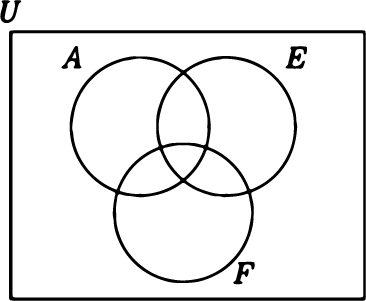
\includegraphics[scale=0.5]{Imagenes/IMG7/Venn1.png}
    \end{center}

    En el primer literal, lo que se nos está solicitando es $| A \cup E \cup F |$ y, al ser conjuntos no disjuntos, se sabe que $ |A \cup E \cup F | \neq |A| + |E| + |F|$, ya que  los  elementos  que  están  en  las  intersecciones  de  los  conjuntos se estarán contando más de una vez.

    Empecemos  a  inlcluir  los  datos  que  conocemos.  En  primer  lugar, el  Universo,  que  es  la  cantidad  de  elementos  encuestados  que  es $|U|=100$ y la triple intersección de los tres conjuntos $ |A \cap E \cap F|=3$, que son los que estudian los tres idiomas.

    Continuamos con las dobles intersecciones, es decir, los alumnos que estudian dos idiomas. Sabemos que hay 10 personas que estudian español y francés ($|E \cap F| =10$), pero en esa zona ya hay 3 estudiantes, entonces para completar los 10 hacen falta 7. De igual forma, se sabe que hay 8 personas que estudian alemán y español ($|A \cap E| =8$), por lo que para completar hacen falta 5 estudiantes, y, por último, para completar los alumnos que estudian alemán y fracés ($|A \cap F| =5$), completamos con 2.

    Continuamos con los conjuntos de cada idioma.  Sabemos que hay 42 personas  que  estudian  francés ($|F|=42$), pero  ya  tenemos  un  total de  12  estudiantes  que  estudian  ese  idioma,  entonces  en  el último espacio se coloca 30.  De manera análoga, para $|A|=30$, se coloca 20 y, para $|E|=28$, se coloca 13.
    
    \begin{center}
        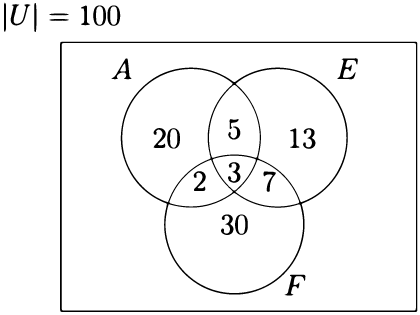
\includegraphics[scale=0.5]{Imagenes/IMG7/Venn3.png}
    \end{center}

    Para responder a la pregunta sumamos todos los datos obtenidos:

    \begin{center}
        $|A \cup E \cup F|=20+2+3+5+13+7+30=80$.
    \end{center}
\end{solucion}

\subsection{Definición}

Para calcular la cardinalidad de $A_1 \cup A_2 \cup ... \cup A_n$ se debe calcular la cardinalidad de todas las posibles intersecciones de conjuntos $A_1, A_2, ..., A_n$, sumar los resultados obtenidos al intersectar un número impar de conjuntos y restar los resultados obtenidos al intersectar un número par de conjuntos.

Los términos “inclusión-exclusión” indican que hay que incluir o sumar las cardinalidades de los conjuntos, después excluir o restar las cardinalidades de las intersecciones de dos conjuntos, luego incluir o sumar las cardinalidades de todas las intersecciones de tres conjuntos, etc., es decir:

\begin{teorema}
    \textbf{Principio de Inclusión-Exclusión}. Dados $n$ conjuntos $A_1, A_2, ..., A_n$, el cardinal de la unión está dado por

    \begin{center}
        $|A_1 \cup A_2 \cup ... \cup A_n| = \displaystyle\sum_{j=1}^{n} (-1)^{j+1} \alpha_j$
    \end{center}
    
    En donde los $\alpha_j$ json las sumas de las cardinalidades de todas las posiles intersecciones de $j$ conjuntos, de la manera siguiente:
    \begin{align*}
        \alpha_1 & = |A_1| + |A_2| + |A_3| + ... + |A_n| \\
        \alpha_2 & = |A_1 \cap A_2| + |A_1 \cap A_3| + |A_1 \cap A_4| + ... + |A_{n-1} \cap A_n| \\
        \alpha_3 & = |A_1 \cap A_2 \cap A_3| + |A_1 \cap A_2 \cap A_4| + |A_1 \cap A_2 \cap A_5| + ... + |A_{n-2} \cap A_{n-1} \cap A_n| \\
        & \ \ \vdots \\
        \alpha_n & = |A_1 \cap A_2 \cap A_3 \cap ... \cap A_n|
    \end{align*}

\end{teorema}

\begin{demostracion}
    Sea $x \ | \ x \in A_1 \cup A_2 \cup ... \cup A_n$, luego se perseguirá que la fórmula del principio de inclusión-exclusión cuente solamente una vez cada elemento en $A_1 \cup A_2 \cup ... \cup A_n$. Ahora, asumiendo que $x \in A_1,A_2,...,A_p$ pero $x \notin A_{p+1},A_{p+2},...,A_n$, entonces $x$ será contado en cada $\alpha_j$ de la siguiente manera:
    \begin{align*}
        \alpha_1 & = p = \binom{p}{1}  \\
        \alpha_2 & = \binom{p}{2} \\
        \alpha_3 & = \binom{p}{3} \\
        & \ \ \vdots \\
        \alpha_p & = \binom{p}{p}
    \end{align*}

    Luego, aplicando la fórmula:

    \begin{center}
        $p-\binom{p}{2}+\binom{p}{3}-\binom{p}{4}+ ... + (-1)^{p-1} \binom{p}{p}$
    \end{center}

    Lo cual equivale a:
    \begin{align*}
        \displaystyle\sum_{j=1}^{p} (-1)^{j+1} \binom{p}{j} & = \displaystyle\sum_{j=1}^{p} (-1)^{j-1} \binom{p}{j} \\
        & = \displaystyle\sum_{j=0}^{p} (-1)^{j-1} \binom{p}{j} + 1 \\
        & = 0 + 1 \\
        & = 1
    \end{align*}

    Con lo cual se puede concluir que el elemento $x$ será contado solo una vez utilizando la fórmula.
\end{demostracion}

En particular, se tiene que

\begin{center}
    $| A \cup B | = |A| + |B| - | A \cap B |$
\end{center}

y que

\begin{center}
    $| A \cup B \cup C | = |A| + |B| + |C| - | A \cap B | - | A \cap C | - | B \cap C | + | A \cap B \cap C |$
\end{center}

\begin{ejemplo}
    Una  clase  de  matemáticas  discreta  contiene  25  estudiantes  en  la clase  con  especialización  en  ciencias  de  la  computación,  13  estudiantes  con  especialización  en  matemáticas  y  8  con especializaciones conjuntas  en  matemáticas  y  ciencias  de  la  computación.  ¿Cuántos estudiantes hay en esta clase, si todos los estudiantes se especializanen  matemáticas,  ciencias  de  la  computación  o  tanto  matemáticas como en ciencias de la computación?
\end{ejemplo}

\begin{solucion}
    Para resolver el ejercicio, utilizamos el principio de inclusión-exclusión para el caso de la unión de dos conjuntos:
    \begin{align*}
        | M \cup C | & = |M| + |C| - | M \cap C | \\
        & = 13 + 25 - 8 \\
        & = 30
    \end{align*}
\end{solucion}

\begin{ejemplo}
    ¿Cómo  podemos  plantear  el  \textbf{problema 3}  de  una  forma  algebraica?
\end{ejemplo}

\begin{solucion}
    Para resolver el ejercicio algebraicamente, utilizamos el principio de inclusión-exclusión para determinar el total de elementos en los tres conjuntos:
    \begin{align*}
        | A \cup E \cup F | & = |A| + |E| + |F| - | A \cap E | - | A \cap F | - | E \cap F | + | A \cap E \cap F | \\
        & = 30 + 28 + 42 - 8 - 5 - 10 + 3 \\
        & = 80
    \end{align*}
\end{solucion}

\newpage

\subsection{Ejercicios}

\begin{ejercicio}
    ¿Cuántos números entre 1 y 6300 inclusive son divisibles entre 3, 5 o 7?
\end{ejercicio}

\begin{ejercicio}
    ¿Cuántos números de tres cifras son divisibles por 2 o 3?
\end{ejercicio}

\begin{ejercicio}
    De los números entre 1 y 200, ¿cuántos no son divisibles entre 4, ni entre 6, ni entre 9?
\end{ejercicio}

\begin{ejercicio}
    ¿De cuántas formas se puede dar una mano de póker (cinco cartas) de modo que contenga al menos una carta de cada palo (considere que el póker tiene 4 palos y 52 cartas)?
\end{ejercicio}

\begin{ejercicio}
    ¿Cuántas cadenas de 9 dígitos tienen al menos una vez cada uno, los dígitos 1, 3 y 7? (Tome en cuenta que una cadena puede ser 000137000, 137777777 o 123456789).
\end{ejercicio}

\begin{ejercicio}
    ¿Cuántos números del 1 al 1000000 no son ni cuadrados perfectos, ni cubos perfectos ni potencias cuartas perfectas?
\end{ejercicio}

\begin{ejercicio}
    Sea $S$ el conjunto de números de 3 dígitos $abc$ tal que $a, b, c \in 1,2, . . . ,9$ y $a,b,c$ son distintos, por lo tanto, $489 \in S$, pero $313 \notin S$ y $507 \notin S$. Encuentre el número de elementos $abc$ en $S$ tal que $a \neq 3$, $b \neq 5$ y $c \neq 7$.
\end{ejercicio}

\begin{ejercicio}
    En un grupo de 30 personas, 10 hablan inglés, 12 hablan castellano y 10 hablan francés. Se sabe que 5 hablan inglés y castellano, 5 castellano y francés, y 7 inglés y francés. Tres personas hablan los tres idiomas. ¿Cuántas personas no hablan ninguno de estos tres idiomas?
\end{ejercicio}

\begin{ejercicio}
    En un grupo de 100 hindués hay 40 que hablan hindi, 40 que hablan bangalí y 20 que hablan panyabí. Hay 20 que hablan hindi y bangalí, y 5 que hablan hindi y panyabí. Hay 31 que hablan al menos dos de estas tres lenguas y 33 que no hablan ninguna de ellas. ¿Cuántos hablan las tres lenguas?
\end{ejercicio}

\section{Desórdenes}

\subsection{Definición}

Si consideramos el orden de los números naturales 1,2,3,4 en la permutación 3142, ningún elemento está en su posición natural. A una permutación con tal propiedad la denominaremos como un \textbf{desorden} o un \textbf{desarreglo}. 

\begin{problema}
    ¿De los 24 posibles ordenamientos de tales números, cuántos desórdenes existen?
\end{problema}

\begin{solucion}
    Denotemos por $D_4$ tal número de desórdenes; por $F_1$, al número de las permutaciones que dejan fijo un elemento en su posición natural; por $F_2$, a las que dejan dos elementos en su posición natural; por $F_3$, a las que dejan tres elemento en su puesto; y por $F_4$, a las que dejan a los 4 elementos en su posición. Así, por el principio de inclusión-exclusión, tenemos el siguiente resultado:

    \begin{center}
        $D_4= 4!-F_1+F_2-F_3+F_4$
    \end{center}

    Ahora bien, $F_1$ se descompone en los que dejan fijo el 1 en su posición, que son 6; los que dejan fijo el 2, que son otras 6; los 6 que dejan el 3; y los 6 que dejan fijo el 4; así, $F_1$ es 24. De las que dejan fijos a dos de los cuatro elementos, están los que dejan fijos el 1 y 2, el 1 y 3, el 1 y 4; los que dejan fijos el 2 y 3, el 2 y 4; y los que dejan fijos el 3 y el 4. Como en cada uno de estos casos, que son seis, el número de permutaciones es 2, resulta que $F_2$ es 12. El caso de que dejen fijos tres elementos contiene los casos  que dejen fijos el 1,2,3; el 1,2,4; el 1,3,4; y el 2,3,4; en total son cuatro casos y cada uno de ellos tiene 1 permutación por lo que $F_3$ es igual a 4. Finalmente, $F_4$ contiene una única permutación, es decir $F_4$ es 1. En resumen tenemos:

    \begin{center}
        $D_4= 24 - 24 + 12 - 4 + 1 = 9$
    \end{center}

    Hay en consecuencia 9 desórdenes en las permutaciones de orden 4.
\end{solucion}

Esta claro que esta relación se puede generalizar.

\subsection{Generalización}

\begin{teorema}
    \textbf{Desórdenes.} En general, se tiene que el total de desórdenes de orden $n$, denotado por $D_n$, es:

    \begin{center}
        $D_n = \displaystyle\sum_{k=0}^{n} (-1)^{k} \binom{n}{k} (n-k)!$
    \end{center}
\end{teorema}

\begin{demostracion}
    El total de permutaciones es $P_n = n!$ Tomando la misma notación del ejemplo anterior, $F_k$ denota aquellas permutaciones que tienen a $k$ (al menos) de sus elementos en la posición que les corresponde; así, el total de permutaciones de $F_k$ lo contamos primero escogiendo los $k$ que quedarán en la posición que les corresponde, lo cuál se puede hacer de $C^k_n$ formas, y luego permutando los restantes $n-k$ objetos, lo que se puede hacer de $P_{n-k}= (n-k)!$ formas; y, por el principio de la multiplicación, $F_k = C^k_n (n-k)!$ Luego, por el principio de inclusión-exclusión:

    \begin{align*}
        D_n & = n!-F_1+F_2-F_3+ ... + (-1)^k F_k + ... + (-1)^n F_n \\
        & = (-1)^0 C^0_n (n-0)! + (-1)^1 C^1_n (n-1)! + (-1)^2 C^2_n (n-2)! + ... + (-1)^n C^n_n (n-n)! \\
        & = \displaystyle\sum_{k=0}^{n} (-1)^{k} \binom{n}{k} (n-k)!
    \end{align*}
\end{demostracion}

Observe que esa expresión se puede manipular algebraicamente y reescribirse como

\begin{center}
    $D_n = n! \displaystyle\sum_{k=0}^{n} \frac{(-1)^{k}}{k!}$
\end{center}

\subsection{Ejercicios}

\begin{ejercicio}
    Calcular $D_3$ y $D_5$.
\end{ejercicio}

\begin{ejercicio}
    Hallar el número de permutaciones de los enteros del 1 al 10 inclusive tal que ningún número esta en su lugar habitual y si en los primeros cinco lugares están

    \renewcommand{\labelenumi}{\alph{enumi})}
    \begin{enumerate}
        \item 1,2,3,4,5; en algún orden.
        \item 6,7,8,9,10; en algún orden.
    \end{enumerate}
\end{ejercicio}

\begin{ejercicio}
    Hallar el número de permutaciones de 1, 2, 3, 4, 5, 6, 7 que no tenga a 1 en el primer lugar, a 4 en el cuarto ni a 7 en el séptimo lugar.
\end{ejercicio}

\begin{ejercicio}
    ¿Cuántas permutaciones de los enteros del 1 al 9 inclusive tienen exactamente tres de sus números en sus posiciones naturales y los otros seis no?
\end{ejercicio}

\begin{ejercicio}
    Se tiene un tablero de 4 × 4 y cuatro colores diferentes. Se pinta cada cuadrito de la primera fila de un color diferente de tal manera que cuando se pinta la segunda fila cada cuadrito es de diferente color al cuadrito de la parte superior. De forma análoga, se colorean las demás filas. ¿De cuántas maneras se puede colorear el tablero?
\end{ejercicio}

\begin{ejercicio}
    En cada uno de los vértices de un cubo hay una mosca. Al sonar un silbato, cada una de las moscas vuela a alguno de los vértices del cubo situado en una misma cara que el vértice dedonde partió, pero diagonalmente opuesto a éste. Al sonar el silbato, ¿de cuántas maneras pueden volar las moscas de modo que en ningún vértice queden dos o más moscas.
\end{ejercicio}

\begin{ejercicio}
    En un campamento se reparten $n$ juguetes diferentes entre $n$ niños. Al día siguiente sevuelven a repartir los mismos juguetes entre los mismos $n$ niños. ¿De cuántas maneras sepueden repartir los juguetes, los dos dias, si ningún niño debe recibir el mismo juguete los dos días?
\end{ejercicio}

\begin{ejercicio}
    $n$ parejas de casados se han reunido para bailar. Si cada caballero tiene la misma probabilidad de bailar con cualquier dama, ¿cuál es la probabilidad de que ningún caballero baile con su propia mujer?
\end{ejercicio}

\begin{ejercicio}
    ¿Cuántas formas hay de que, entre 10 clientes, ninguno reciba su propio sombrero si el empleado de guardaropa devuelve los sombreros al azar?
\end{ejercicio}

\begin{ejercicio}
    Supongamos que tenemos que asignar asientos a un grupo de $n$ estudiantes para dos clases distintas en la misma aula. ¿De cuántas formas se puede hacer si no queremos que ningún estudiante esté sentado en el mismo sitio en las dos clases?
\end{ejercicio}

\begin{ejercicio}
    Se tienen 5 sobres y 5 cartas y se distribuyen al azar las cartas en los sobres (solo una carta le corresponde a cada sobre).

    \renewcommand{\labelenumi}{\alph{enumi})}
    \begin{enumerate}
        \item ¿De cuántas formas se pueden distribuir para que no haya coincidencia?
        \item ¿De cuántas formas para que haya una coincidencia?
        \item ¿Y para que haya exactamente dos coincidencias?
        \item ¿De cuántas formas para que haya tres coincidencias?
        \item ¿De cuántas formas para que haya cuatro coincidencias?
        \item ¿De cuántas formas para que haya cinco coincidencias?
    \end{enumerate}
\end{ejercicio}

\end{document}